\documentclass[twoside,11pt]{article}

\usepackage{jagi}
\usepackage{times}
\usepackage{amsmath}
\usepackage{booktabs}
\usepackage{graphicx}
\usepackage{float}
\usepackage{caption}
\usepackage{tabularx}
\usepackage{array}
\usepackage{tikz}
\usepackage{pgfplots}
\usepackage{pgf-pie}
\usepackage[section]{placeins}
\pgfplotsset{compat=1.18}
\counterwithin{table}{section}
\setlength{\parindent}{0pt}
\setlength{\parskip}{0pt}
\setlength{\abovedisplayskip}{6pt}
\setlength{\belowdisplayskip}{6pt}
\setlength{\abovedisplayshortskip}{4pt}
\setlength{\belowdisplayshortskip}{4pt}
\raggedbottom

\newcommand{\dataset}{{\cal D}}
\newcommand{\fracpartial}[2]{\frac{\partial #1}{\partial #2}}


\makeatletter
\providecommand{\@startauthor}{\noindent\normalsize\bfseries}
\providecommand{\@endauthor}{}
\makeatother

\firstpageno{1}

\begin{document}

\title{
El Problema del Agente Viajero mediante Recocido \\ Simulado por Aceptación de Umbrales
}

\author{
    \name Michelle Ariadna García Díaz \\
    \addr Universidad Nacional Autónoma de México \\
    Facultad de Ciencias \\
    Seminario de Optimización de Heurísticas Combinatorias
}

\editor{}

\maketitle

\begin{abstract}
En este trabajo se aborda una variante del Problema del Agente Viajero (TSP), en la que se busca una ruta de bajo costo que recorra un conjunto de ciudades sin requerir que la ciudad final coincida con la inicial. Para ello se implementó en Nim una heurística de recocido simulado basada en aceptación por umbrales, cuyo objetivo es encontrar soluciones suficientemente buenas sin garantizar el óptimo global. La implementación utiliza permutaciones de ciudades, generación de vecinos, evaluación incremental del costo y semillas pseudoaleatorias para favorecer la reproducibilidad. Finalmente, se realizan múltiples corridas y experimentos con diferentes configuraciones de parámetros para analizar el comportamiento de la heurística y la calidad de las soluciones obtenidas.

\end{abstract}



\section{Introducción}
La optimización combinatoria estudia problemas en los que se busca encontrar una solución que optimice una función objetivo dentro de un conjunto de posibles soluciones. En muchos de estos problemas, el número de soluciones crece rápidamente conforme aumenta el tamaño de la entrada, lo que hace casi imposible para los humanos la búsqueda exhaustiva de una solución óptima. \\

Uno de los problemas clásicos dentro de esta área es el Problema del Agente Viajero (\textit{Traveling Salesman Problem}, TSP). De manera general, este problema busca determinar un orden para visitar un conjunto de ciudades de forma que el costo total del recorrido sea mínimo. En esta implementación se considera una variante en la que cada ciudad debe ser visitada una sola vez, pero no se exigue regresar a la ciudad inicial al finalizar el recorrido- Por lo tanto, una solución correspode a un camino que vista todas las ciudades de la instancia. Para abordar este problema se utiliza la metaheurística de Aceptación por Umbrales (\textit{Threshold Accepting}), propuesta por Gunter Dueck y Tobias
Scheuer en 1990. \\

El espacio de búsqueda de las soluciones esta dado por las distintas permutaciones, de las ciudades que componen una instancia, lo cual temina en el factorial del número de ciudades de la instancia. Debido al rápido crecimiento de este espacio conforme aumenta el número de ciudades, realizar una exploración completa resulta prácticamente imposible y poco práctico para instancias de un tamalo considerable. Una alternativa es utilizar heurísticas, que permiten explorar el espacio de soluciones en busca de soluciones de 'buena' calidad sin realizar una búsqueda completa, sin embargo en estas es imposible garantizar la obtención del ótimo global.\\

En este proyecto, realizado para el Seminario de Optimización de Heurísticas Combinatorias, se aborda la variante del TSP mencionada anteriormente. Aunque esta variante no corresponde al problema original, tiene diversas aplicaciones prácticas en el mundo real, como, por ejemplo, los sistemas de envío y reparto de paquetería. \\

Este problema y la heurística utilizada fueron implementados en el
lenguaje de programación Nim. Además de la implementación, se realizó una etapa de experimentación mediante el uso de semillas pseudoaleatorias y la modificación de distintos parámetros de configuración, los cuales se describirán más adelante en el reporte. La experimentación se llevó a cabo mediante múltiples corridas con diferentes configuraciones, con el propósito de observar el comportamiento de la heurística y analizar la calidad de las soluciones
obtenidas. Los experimentos se realizaron sobre dos instancias del problema: una compuesta por 40 ciudades y otra por 150 ciudades. 


\section{Problema}

Como se mencionó anteriormente el problema abordado en este proyecto corresponde a una variante del Problema del Agente Viajero (TSP). Dado un subconjunto de ciudades en un mapa, se busca
encontrar una trayectoria de costo mínimo que pase por todas ellas, si dicha
trayectoria existe. A diferencia del TSP clásico, en esta variante no se exige
regresar a la ciudad inicial al finalizar el recorrido.\\

El problema considerado se representa mediante una gráfica ponderada $G=(V,E)$, donde los vértices representan ciudades, las aristas representan las conexiones existentes entre ellas y su peso corresponde a la distancia entre cada par de ciudades. Una instancia $S\subseteq V$ está formada por las ciudades que se desean visitar.\\

Una solución $P$ corresponde a una permutación de las $k$ ciudades de la
instancia,

\[
P=(v_{\rho(1)},v_{\rho(2)},\ldots,v_{\rho(k)}).
\]

La solución es factible cuando todas las conexiones entre ciudades consecutivas existen en la gráfica original. Debido a que se considera una variante abierta del TSP, únicamente se consideran las $k-1$ conexiones consecutivas.\\

Para poder evaluar cualquier permutación, las conexiones inexistentes reciben un peso aumentado $w_S$, calculado a partir de la distancia natural entre las ciudades y la distancia máxima de la instancia. De esta manera, si la solución tiene una conexión inexistente en penalizada.

\[
w_S(u,v)=
\begin{cases}
w(u,v), & \text{si } (u,v)\in E,\\[4pt]
d(u,v)\cdot \max d(S), & \text{en otro caso}.
\end{cases}
\]

\vspace{0.05cm}

Finalmente, las soluciones se evalúan mediante la función de costo 

\[
f(P)=
\frac{\displaystyle\sum_{i=2}^{k}
w_S(v_{\rho(i-1)},v_{\rho(i)})}
{N(S)},
\]

donde $N(S)$ es la suma de las $k-1$ aristas de mayor peso de la instancia, que actuia como normalizador.
Esta normalización permite que las soluciones factibles tengan una evaluación entre $0$ y $1$, mientras que las no factibles obtienen una evaluación mayor que $1$. El objetivo del problema consiste en minimizar $f(P)$.


\section{Heurística}

Para buscar soluciones para el problema se utiliza Aceptación por Umbrales (\textit{Threshold Accepting}), una variante del Recocido Simulado. La heurística parte de una solución $s$ y una temperatura $T$, y genera de manera pseudoaleatoria una solución vecina $s'$. Esta solución se acepta cuando

\[
f(s') \leq f(s)+T.
\]

Por lo tanto, además de aceptar soluciones que mejoran el costo actual, se pueden aceptar soluciones que empeoran. Esto permite explorar ampliamente el espacio de búsqueda y disminuir la posibilidad de permanecer en
un mínimo local. Conforme avanza la ejecución, la temperatura se reduce mediante

\[
T\leftarrow\phi T, \qquad 0<\phi<1,
\]

hasta alcanzar un valor menor que  un $\varepsilon$.\\

Las soluciones aceptadas se organizan en lotes de tamaño $L$. Para cada temperatura se procesan lotes mientras se mantenga la condición de equilibrio térmico, utilizando además un número máximo de intentos para evitar que la búsqueda permanezca indefinidamente  y se 'estanque' nuestro programa intentando completar un lote. Durante toda la ejecución se conserva la mejor solución encontrada.\\

La temperatura inicial puede establecerse directamente o determinarse mediante una búsqueda que intenta alcanzar una proporción objetivo $P$ de vecinos aceptados. Más adelante veremos que en la implementación se tiene la opción de elegir mediante que variante queremos realizar un experimento. Para cada corrida utiliza una semilla, permitiendo reproducir los experimentos utilizando los mismos parámetros, la reproducibilidad es fundamental para este tipo de problemas.

\section{Diseño de la solución}

La solución fue diseñada separando el problema en distintos componentes: lectura de datos, representación de la gráfica, evaluación de soluciones, generación de vecinos, ejecución de la heurística y experimentación. Esta separación permite mantener independientes la representación del TSP y el funcionamiento de Aceptación por Umbrales.\\

Al iniciar una ejecución se cargan las ciudades y conexiones almacenadas en la base de datos, así como las ciudades correspondientes a la instancia. A partir
de esta información se construye la gráfica y se calculan previamente los valores necesarios para evaluar las soluciones, como la distancia máxima, el normalizador y los pesos aumentados.\\

Una solución se representa mediante una permutación de los índices de las ciudades de la instancia. Para generar una solución vecina se seleccionan aleatoriamente dos índices distintos de la permutación y se intercambian los elementos ubicados en dichas posiciones. \\

Cada vecino se evalúa utilizando el criterio de Aceptación por Umbrales. Si es aceptado, se conserva el intercambio y la solución vecina pasa a ser la nueva
solución actual; en caso contrario, el intercambio se revierte. Durante toda la corrida se conserva también la mejor solución encontrada.\\

Finalmente, el sistema permite realizar múltiples corridas utilizando distintas semillas pseudoaleatorias y conservar el mejor resultado obtenido.

\section{Detalles de la implementación}

El sistema fue implementado en el lenguaje de progrmación Nim siguiendo principalmente un paradigma procedimental y modular. El proyecto se dividió en módulos con responsabilidades específicas, manteniendo separadas la persistencia de datos, la representación
del TSP, la heurística y la ejecución de experimentos.

\subsection{Arquitectura}

La estructura principal del proyecto es:

\begin{figure}[H]
\centering

\begin{minipage}[t]{0.47\textwidth}
\begin{verbatim}
tsp/
|-- data/
|   |-- tsp.db
|   `-- instances/
|       |-- input-40.tsp
|       `-- input-150.tsp
|-- scripts/
|-- src/
|   |-- main.nim
|   |-- models/
|   |-- persistence/
|   |-- tsp/
|   |-- heuristics/
|   |   `-- threshold_acceptance/
|   `-- runner/
`-- tests/
\end{verbatim}
\end{minipage}
\hfill
\begin{minipage}[t]{0.47\textwidth}
\small
Los módulos de \texttt{models} contienen las estructuras utilizadas para representar los datos; \texttt{persistence} se encarga de obtenerlos desde SQLite y los archivos de instancia; \texttt{tsp} contiene las operaciones específicas del problema; \texttt{heuristics} implementa Aceptación por Umbrales; y \texttt{runner} administra las múltiples corridas experimentales.
\end{minipage}
\caption{Organización de los principales módulos del sistema.}
\label{fig:project-structure}
\end{figure}

\subsection{Representación de los datos}

La información original se almacena en SQLite mediante dos entidades principales: ciudades y conexiones. En Nim estos registros se representan mediante los tipos \texttt{City} y \texttt{Connection}. \\

Las conexiones recuperadas de la base de datos se utilizan para construir una matriz de adyacencia. Una de las desiciones de optimización tomada fue que las matrices se almacenan internamente mediante una secuencia unidimensional, donde el elemento $(i,j)$ se encuentra en $i\cdot n+j$. Esta representación permite almacenar los datos de manera contigua y realizar accesos directos durante las evaluaciones.

\subsection{Desacoplamiento de la heurística}

Una de las principales decisiones de diseño fue evitar que Aceptación por Umbrales dependiera del tipo \texttt{City} o de cualquier característica particular del TSP. Para ello se utilizaron los genéricos de Nim:

\begin{figure}[H]
\centering

\begin{minipage}[t]{0.38\textwidth}
\begin{verbatim}
proc thresholdAcceptance[T](
    solution: var seq[T],
    ...
)
\end{verbatim}
\end{minipage}
\hfill
\begin{minipage}[t]{0.57\textwidth}
\small
La heurística trabaja con soluciones de tipo \texttt{seq[T]} y las operaciones específicas del problema son proporcionadas mediante funciones. Por lo tanto, la implementación de Aceptación por Umbrales no necesita conocer ciudades, coordenadas, conexiones ni la forma en que se calcula el costo.
\end{minipage}

\caption{Uso de tipos genéricos para desacoplar la heurística del TSP.}
\label{fig:generic-threshold}
\end{figure}

En este proyecto, una solución del TSP se representa mediante

\[
\texttt{seq[int]},
\]

donde los enteros corresponden a los índices utilizados para consultar las matrices. Sin embargo, el tipo genérico \texttt{T} permite que la heurística pueda reutilizarse posteriormente con otras representaciones y otros problemas de optimización.

\subsection{Configuración de la temperatura inicial}

La implementación permite establecer la temperatura inicial de dos maneras. La primera consiste en proporcionar manualmente un valor para $T$, que se
utiliza directamente al comenzar la heurística.

La segunda opción realiza una búsqueda automática de la temperatura inicial. 

\begin{verbatim}
--temperature:50000
--search-temperature:true
--target-acceptance:0.85
\end{verbatim}

\subsection{Decisiones de optimización}

Para la experimentación se presentaron algunas dificultades, ya que durante las primeras etapas el sistema requería demasiado tiempo para procesar las
semillas. Por esta razón, no solo al inicio, sino también a lo largo de la experimentación, se realizaron distintas modificaciones al sistema con el objetivo de reducir los tiempos de ejecución. Las optimizaciones que tuvieron un mayor impacto fueron:

\begin{itemize}
    \setlength{\itemsep}{1pt}
    \setlength{\parskip}{0pt}
    \setlength{\parsep}{0pt}

    \item Precalcular los pesos aumentados antes de iniciar la heurística.
    \item Representar las soluciones mediante índices enteros en lugar de  estructuras completas de tipo \texttt{City}.
    \item Almacenar las matrices mediante memoria contigua.
    \item Calcular incrementalmente el costo de un vecino considerando únicamente las aristas afectadas por el intercambio.
    \item Mantener el costo actual durante la ejecución para evitar evaluaciones completas innecesarias.
\end{itemize}

Finalmente, el módulo \texttt{runner} mantiene separada la experimentación de la heurística. Este módulo permite realizar múltiples corridas con semillas distintas mediante un script y conservar la mejor solución, su costo y la semilla que permitió obtenerla para posteriormente poder reproducir el experimento.

\section{Experimentación y resultados}

La experimentación se realizó sobre dos instancias del problema, una de 40 ciudades y otra de 150 ciudades. Debido al carácter pseudoaleatorio de la heurística, cada corrida fue identificada mediante una semilla, permitiendo reproducir posteriormente aquellas ejecuciones que produjeran resultados de interés.\\

La afinación de los parámetros se realizó de manera experimental. A lo largo del desarrollo se probaron distintas combinaciones del tamaño de lote, factor
de enfriamiento, número máximo de intentos, número máximo de lotes y temperatura inicial. La instancia de 150 ciudades fue utilizada principalmente para esta etapa, debido a que presentó una mayor dificultad para encontrar soluciones factibles y de bajo costo. Ya al final una vez teniendo mas claro el manejo de los parámetros, se experimento en la de 40 para llegar a \texttt{0.2638}, lo que \textit{se cree que es el óptimo}.  Durante ese proceso fue de gran ayuda la discusión en clase del Seminario, ya que ayudo a guíar los parémetros de la experimentación. 


\subsection{Experimentos}

La experimentación no consistió en modificar un único parámetro de manera aislada, sino en probar distintas configuraciones conforme se observaba el comportamiento del sistema, al prinicpio fue \textit{muy} complicado inclusive obtener soluciones factibles ya que no se tenía idea de cuales eran los valores de ciertos parametros, por ello recalco que la disución en grupo fue muy importante. Por esta razón, los resultados siguientes deben interpretarse como hitos del proceso de afinación y no como una comparación controlada entre parámetros individuales, además no fueron 6 etepas numerables, solo se resumen los momentos donde empezó a haber una disminución importante en la evaluación de costo.\\

En las primeras ejecuciones sobre la instancia de 150 ciudades era común obtener soluciones no factibles. Conforme se modificaron los parámetros y se optimizó la implementación, comenzaron a encontrarse soluciones factibles con mayor frecuencia y con evaluaciones progresivamente menores.

\begin{table}[H]
\centering

\footnotesize
\renewcommand{\arraystretch}{1.15}
\setlength{\tabcolsep}{5pt}

\begin{tabular}{|c|p{8.2cm}|c|}
\hline
\textbf{Etapa} &
\textbf{Característica de la configuración} &
\textbf{Mejor $f(P)$ observada} \\ \hline

1
& Primeras soluciones factibles
& 0.2219802903 \\ \hline

2
& Ajustes en tamaño de lote y número de intentos
& 0.1788749280 \\ \hline

3
& Enfriamiento más lento
& 0.1630968209 \\ \hline

4
& Nuevos ajustes de $\epsilon$ y lotes
& 0.1458996316 \\ \hline

5
& Búsqueda automática de temperatura
& 0.1414718286 \\ \hline

6
& Configuración final
& \textbf{0.1382118879} \\ \hline

\end{tabular}

\caption{Algunos hitos durante la experimentación con 150 ciudades.}
\label{tab:experiment-evolution}

\end{table}



Un aspecto importante observado durante esta etapa además del tiempo fue la factibilidad. En una de las configuraciones intermedias de 100 corridas únicamente se obtuvieron 6 soluciones factibles, mientras que en experimentos posteriores después de sintonizar un poco mejor el sistema se registraron bloques  completos de $95/100$ corridas factibles. Esto mostró que los parámetros no solamente afectaban la calidad de la mejor solución, sino también la capacidad del sistema para terminar en regiones factibles del espacio de búsqueda.
Los parámetros que mas influyeron al ajustar fueron \textit{número máximo de intentos}, \textit{tamaño de lote} y \textit{factor de enfriamiento}, se tuvo un cambio radical en esta. \\


\begin{figure}[H]
    \centering

    \begin{minipage}[t]{0.48\linewidth}
        \centering
        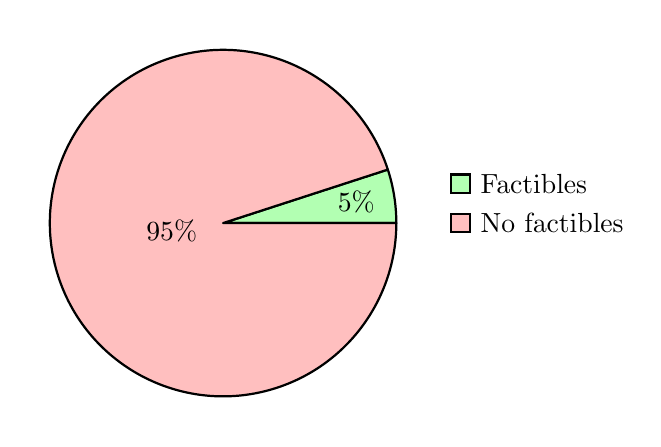
\begin{tikzpicture}
            \pie[
                radius=2.2,
                text=legend,
                color={green!30, red!25}
            ]{
                5/Factibles,
                95/No factibles
            }
        \end{tikzpicture}
        \caption*{(a) Configuración inicial: 5\% de soluciones factibles.}
    \end{minipage}
    \hfill
    \begin{minipage}[t]{0.48\linewidth}
        \centering
        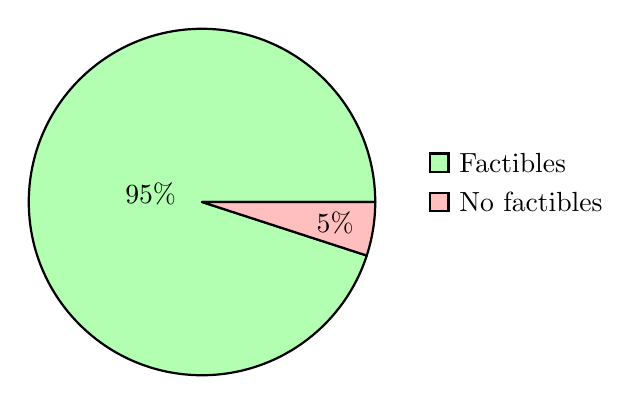
\begin{tikzpicture}
            \pie[
                radius=2.2,
                text=legend,
                color={green!30, red!25}
            ]{
                95/Factibles,
                5/No factibles
            }
        \end{tikzpicture}
        \caption*{(b) Configuración ajustada: 95\% de soluciones factibles.}
    \end{minipage}

    \caption{Comparación del porcentaje de factibilidad obtenido en la instancia de 150 ciudades antes y después del ajuste de parámetros.}
    \label{fig:factibilidad-pasteles}
\end{figure}


Como se mencionó el tiempo también fue un factor muy importante durante la  experimentación. A continuación una tabla de como este fue diminuyendo de acuerdo a las optimizaciones realizadas. 

\begin{table}[H]
\centering

\footnotesize
\renewcommand{\arraystretch}{1.15}
\setlength{\tabcolsep}{4pt}

\begin{tabularx}{\linewidth}{
    |c|
    X|
    >{\centering\arraybackslash}p{2.5cm}|
}
\hline

\textbf{Etapa} &
\textbf{Optimización incorporada} &
\textbf{Tiempo aprox. por semilla} \\ \hline

1
& Implementación inicial, sin optimizaciones
& $\sim$30 min \\ \hline

2
& Evitar recalcular completamente la función de costo para cada vecino
& $\sim$15 min \\ \hline

3
& Precalcular valores utilizados durante la evaluación, como los pesos aumentados
& $\sim$12 min \\ \hline

4
& Representar las matrices mediante memoria contigua
& $\sim$8 min \\ \hline

5
& Representar las soluciones como \texttt{seq[int]} en lugar de
\texttt{seq[City]}
& $\sim$1 min 15 s \\ \hline

\end{tabularx}

\caption{Evolución aproximada del tiempo de ejecución por semilla después de
incorporar distintas optimizaciones.}
\label{tab:optimization-times}
\end{table}


\subsection{Configuración experimental}

Para la instancia de 150 ciudades se paralelizaron las
corridas mediante cuatro procesos independientes, asignando a cada uno un intervalo diferente de semillas. Las semillas s edividian entre los 4 procesos, y depués de eso para la siguiente semilla se le sumaba uno a la anterior. La configuración con la que se obtuvieron los mejores resultados para cada instancia se presenta en la Tabla~\ref{tab:final-config}.

\begin{table}[H]
\centering

\footnotesize
\renewcommand{\arraystretch}{1.15}
\setlength{\tabcolsep}{5pt}

\begin{tabular}{|p{5.7cm}|c|c|}
\hline
\textbf{Parámetro} &
\textbf{40 ciudades} &
\textbf{150 ciudades} \\ \hline

Corridas
& 300
& 500 \\ \hline

Procesos
& 4
& 4 \\ \hline

Semilla
& 28973189451
& 9433578794396893 \\ \hline

Valor inicial de $T$
& 50000
& 50000 \\ \hline

Búsqueda de temperatura
& Sí
& Sí \\ \hline

Aceptación objetivo $P$
& 0.85
& 0.85 \\ \hline

$\varepsilon$
& $0.00001$
& $0.00001$ \\ \hline

Factor de enfriamiento $\phi$
& 0.975
& 0.995 \\ \hline

Tamaño de lote $L$
& 700
& 4000 \\ \hline

Intentos máximos
& 16000
& 75000 \\ \hline

Lotes máximos por temperatura
& 50
& 50 \\ \hline

\end{tabular}
\caption{Configuraciones utilizadas para los mejores resultados obtenidos.}
\label{tab:final-config}
\end{table}

Lla búsqueda automática de temperatura se encontraba habilitada, el valor $T=50000$ funcionó como valor inicial para el procedimiento de búsqueda de temperatura. 



\subsection{Resultados}

\subsubsection{Instancia de 150 ciudades}

El mejor resultado obtenido para la instancia de 150 ciudades fue

\[
\boxed{f(P)=0.13821188785057265}
\]

utilizando la semilla

\[
\boxed{9433578794396893}.
\]

Esta solución apareció en el proceso 0 durante la corrida 117 de las 125 asignadas a dicho proceso. Hasta ese momento se habían obtenido 115 soluciones factibles de las 117 corridas realizadas por ese proceso.

\begin{center}
    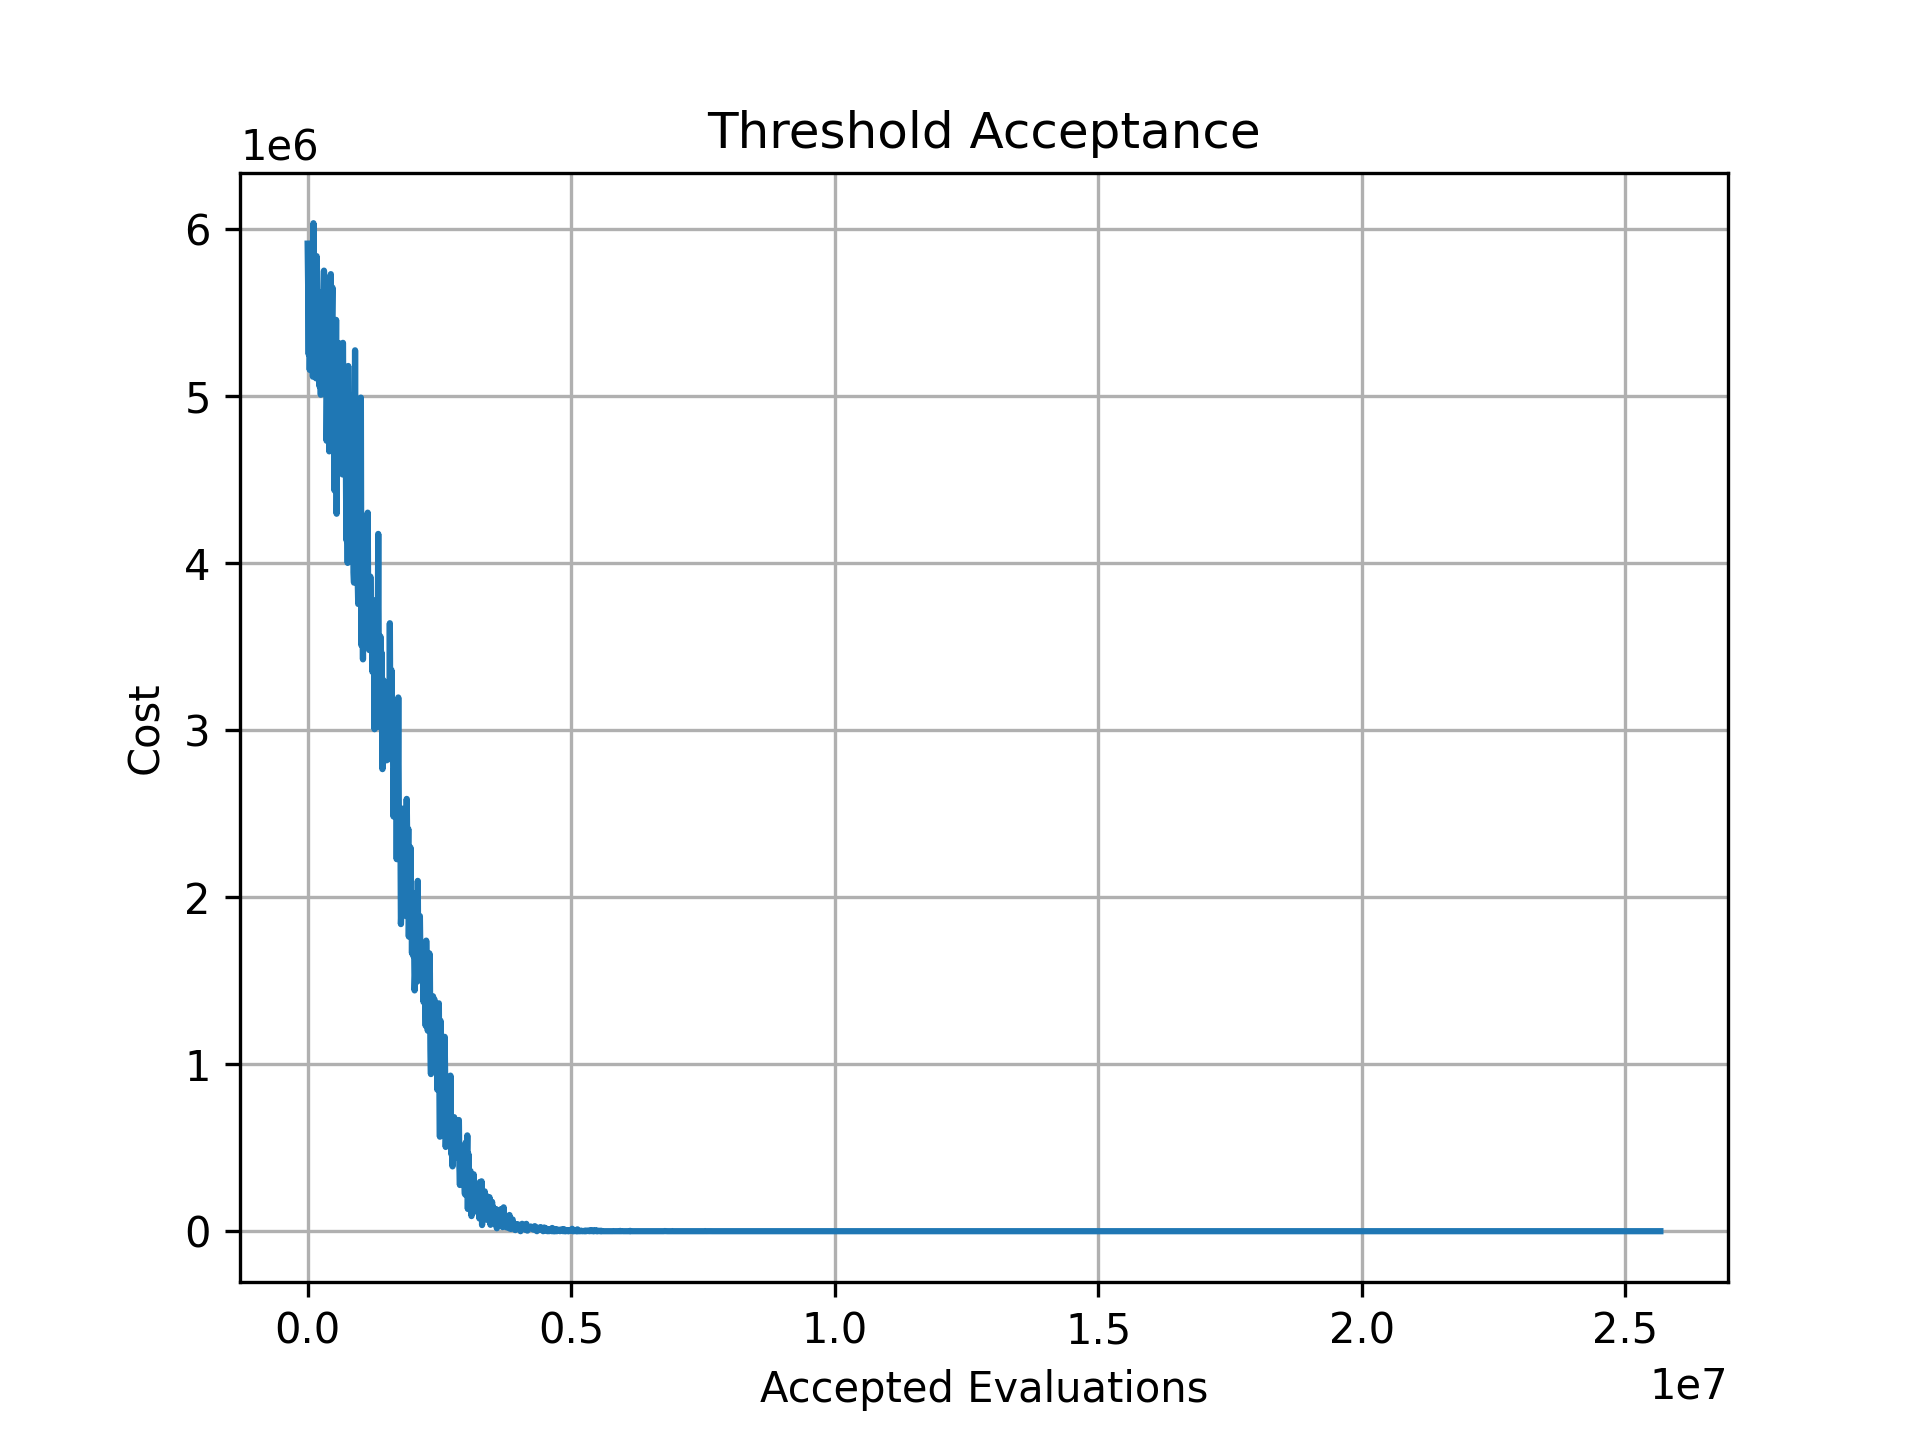
\includegraphics[
        width=0.90\linewidth,
        height=0.42\textheight,
        keepaspectratio
    ]{figures/eval150.png}

    \captionof{figure}{Evolución de la función de evaluación para la semilla 9433578794396893.}
    \label{fig:evaluacion-150}
\end{center}

\begin{center}
    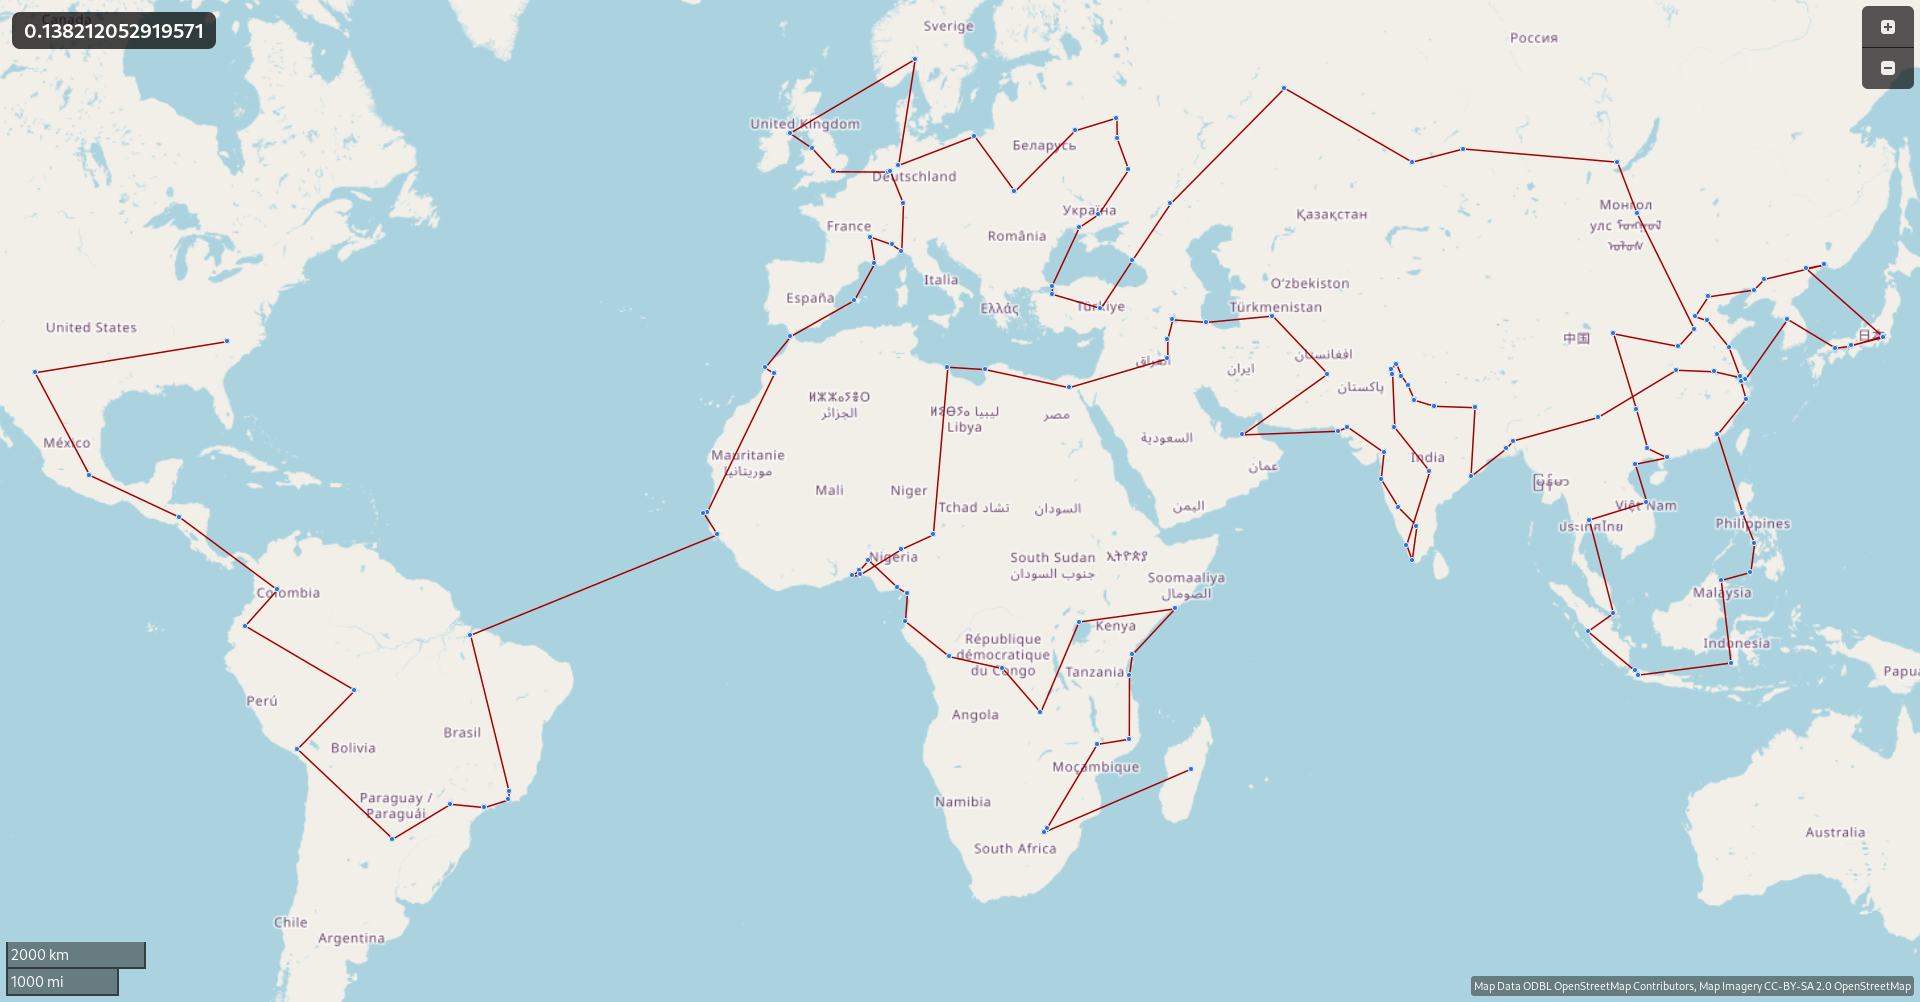
\includegraphics[
        width=0.80\linewidth,
        height=0.32\textheight,
        keepaspectratio
    ]{figures/mapa150.png}

    \captionof{figure}{Visualización de la ruta obtenida para 150 ciudades. Mapa generado por Ianluck Peña.}
    \label{fig:ruta-150}
\end{center}

La ruta correspondiente fue:

\begin{center}
\begin{minipage}{0.96\linewidth}
\scriptsize\ttfamily
171, 652, 1075, 483, 512, 821, 75, 346, 77, 183, 179, 671, 16, 520, 186, 675, 340, 502, 828, 12, 1038, 339, 244, 826, 444, 17, 25, 492, 491, 499, 347, 817, 489, 4, 174, 165, 3, 333, 27, 353, 990, 981, 988, 23, 176, 668, 352, 978, 5, 6, 1004, 351, 991, 185, 22, 676, 673, 173, 2, 9, 832, 661, 663, 657, 829, 1, 986, 508, 168, 505, 19, 496, 839, 815, 184, 667, 656, 507, 7, 823, 678, 816, 187, 982, 14, 181, 332, 345, 820, 26, 654, 490, 653,
344, 665, 163, 172, 182, 329, 509, 493, 979, 837, 995, 984, 501, 164, 11, 1003, 349, 331, 662, 8, 999, 334, 674, 985, 343, 510, 660, 20, 825, 500, 504, 511, 327, 670, 350, 840, 336, 980, 297, 1001, 74, 822, 166, 658, 666, 818, 655, 819, 330, 1073, 169, 1037, 326, 328, 167, 495, 494
\end{minipage}
\end{center}


\subsubsection{Instancia de 40 ciudades}

Para la instancia de 40 ciudades se obtuvo como mejor evaluación

\[
\boxed{f(P)=0.2638196076095546}.
\]

En este caso fue mas sencilló ya conociendo un poco mejor el manejo de lo parámetro. Se realizó una corrida con la semilla \texttt{28973189451}. La configuración utilizada fue de menor tamaño que la empleada para la instancia de 150 ciudades, utilizando lotes de 700 soluciones aceptadas y un máximo de 16000 intentos.

\begin{center}
    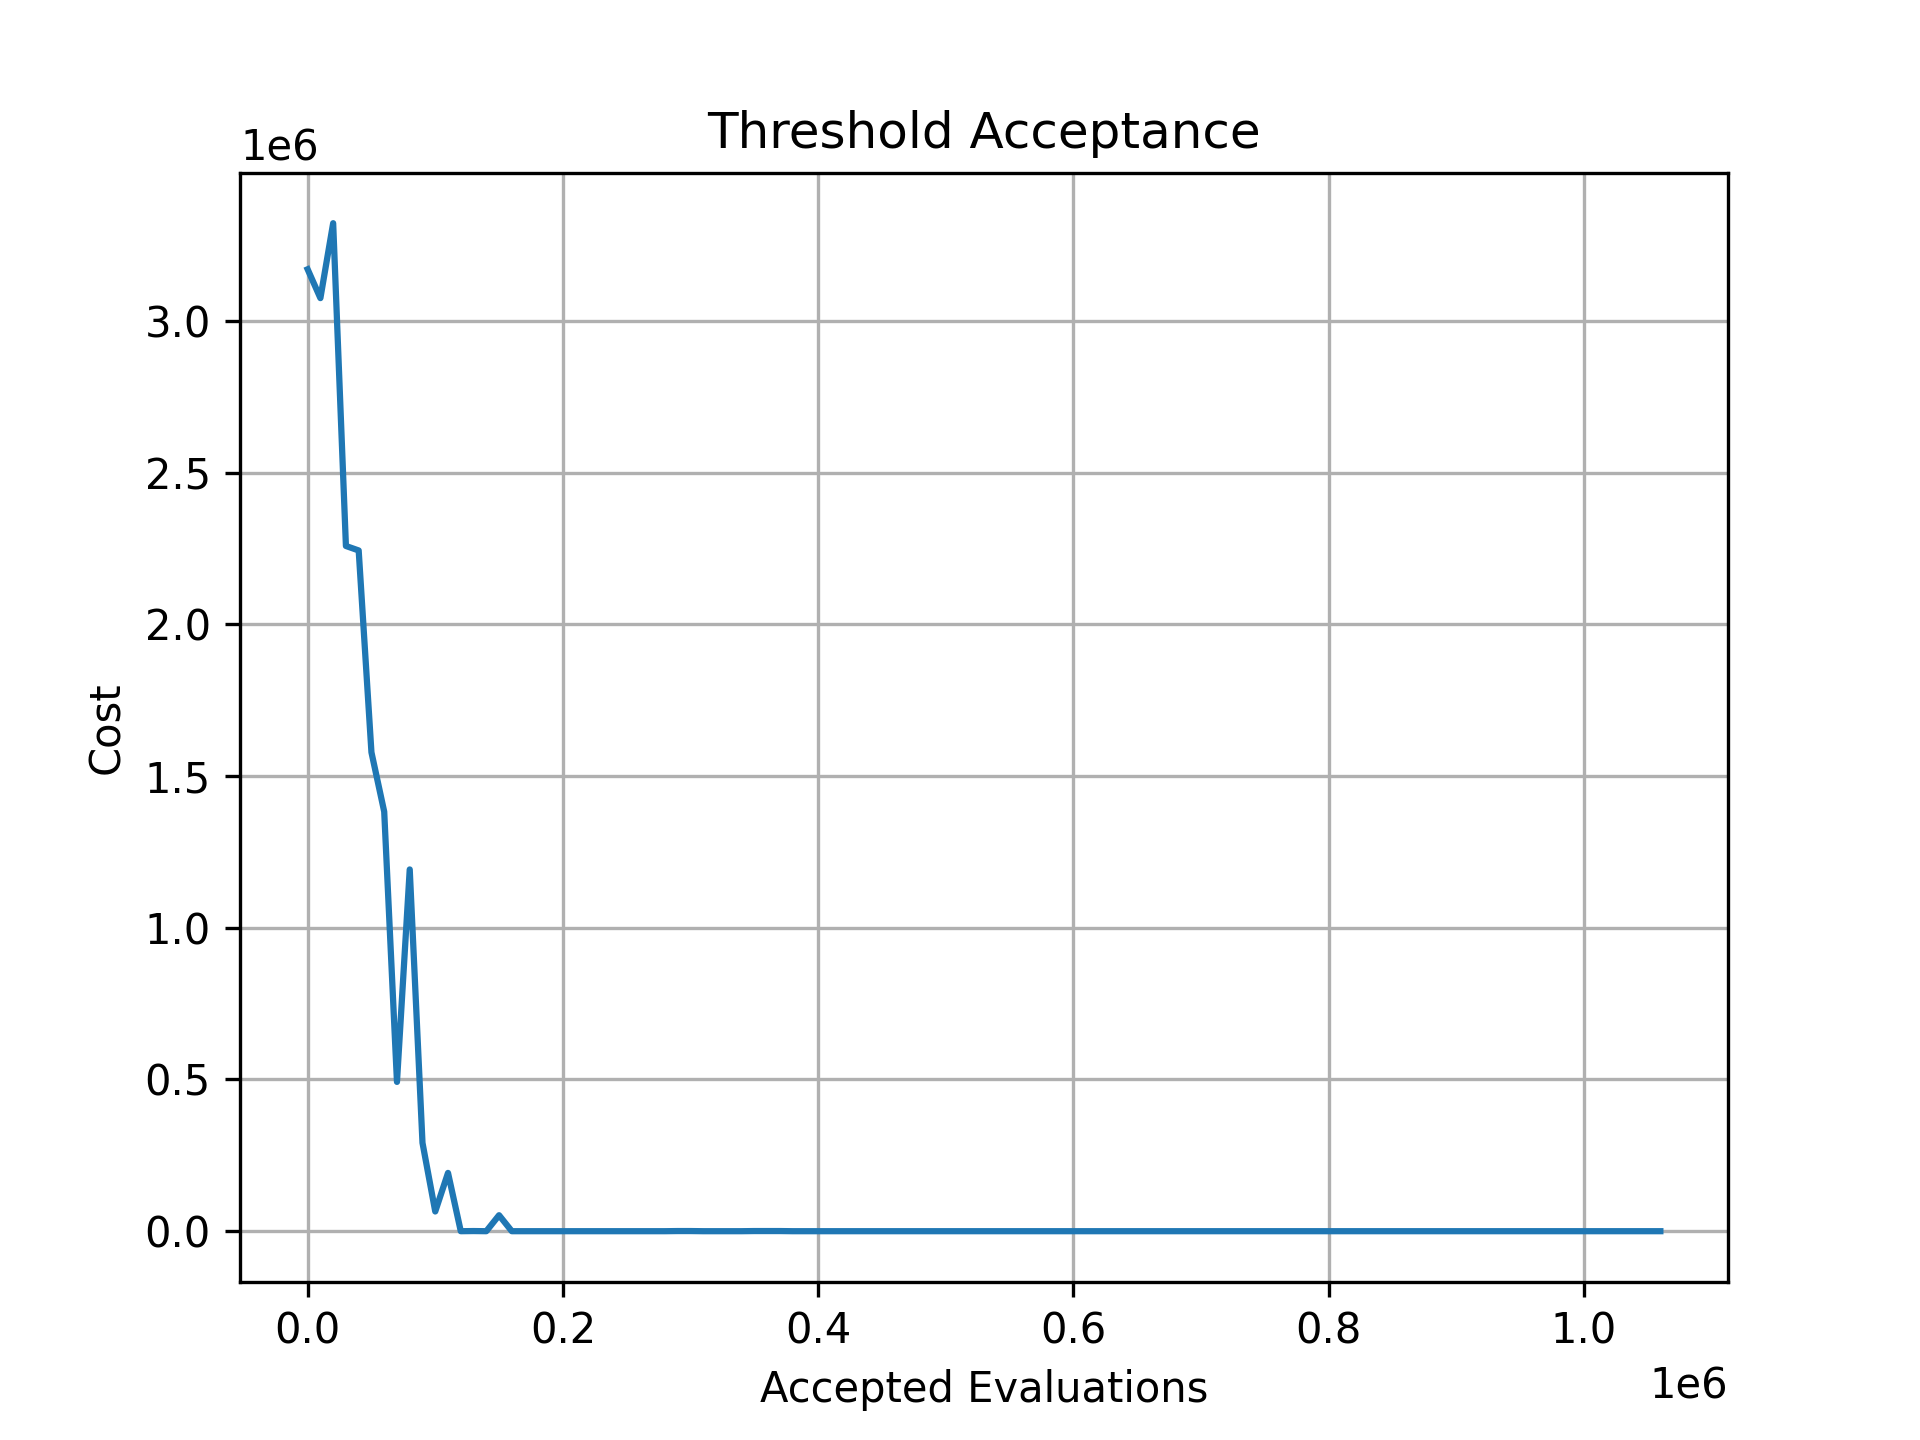
\includegraphics[
        width=0.90\linewidth,
        height=0.42\textheight,
        keepaspectratio
    ]{figures/eval40.png}

    \captionof{figure}{Evolución de la función de evaluación para la semilla 28973189451.}
    \label{fig:evaluacion-40}
\end{center}

\begin{center}
    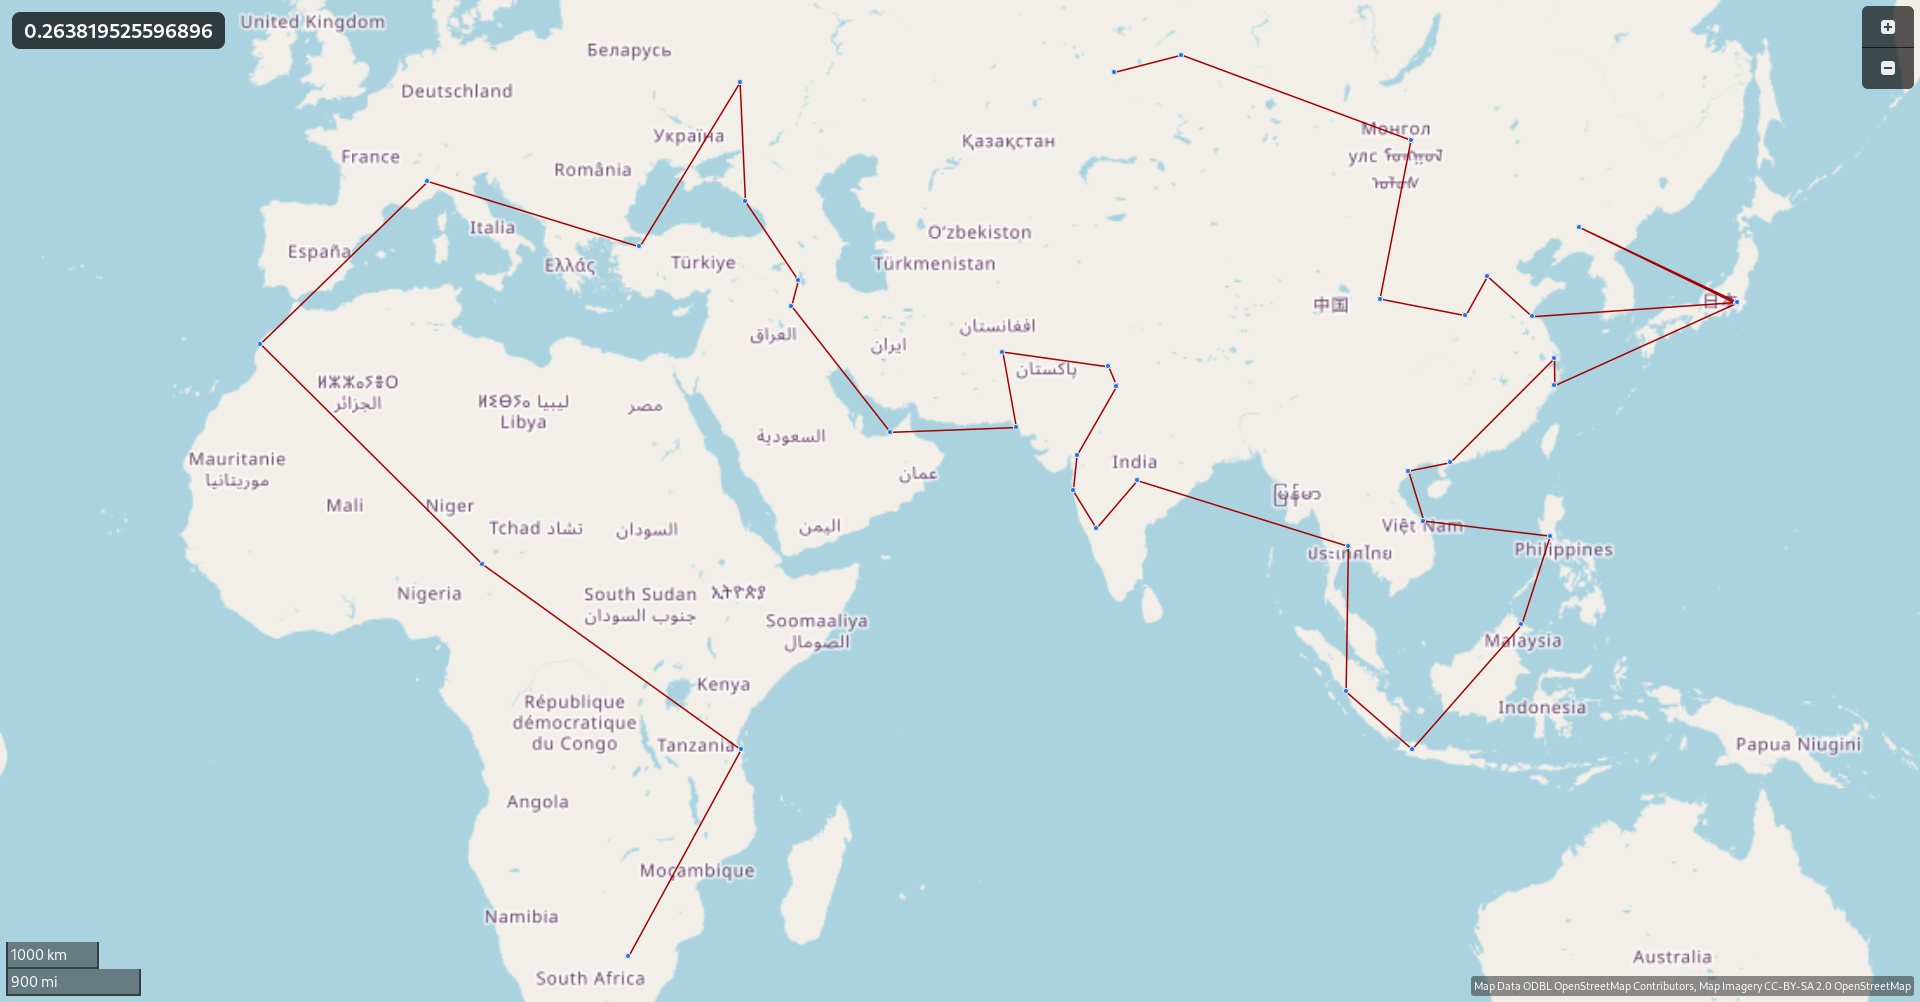
\includegraphics[
        width=0.80\linewidth,
        height=0.32\textheight,
        keepaspectratio
    ]{figures/mapa40.png}

    \captionof{figure}{Visualización de la ruta obtenida para 40 ciudades. Mapa elborado por Ianluck Peña}
    \label{fig:ruta-40}
\end{center}


\subsection{Análisis de resultados}

Los resultados muestran que la instancia de 150 ciudades fue más sensible a la configuración de parámetros, ya que en las primeras etapas se obtenían con frecuencia soluciones no factibles y evaluaciones muy altas debido a las conexiones penalizadas. A lo largo de la experimentación se logró aumentar la factibilidad a casi un $100\%$ y reducir progresivamente el costo, los factores de configuración que mas afectaron fueron: el temaño de lote, el factor de enfriamento, número máximo de intentos y $\epsilon$. De igual forma, las mejores soluciones se obtuvieron posteriormente con la búsqueda automática de temperatura y configuraciones más ajustadas, alcanzando finalmente una evaluación de $0.13821188785057265$ para 150 ciudades. En la instancia de 40 ciudades se obtuvo una evaluación de $0.2638196076095546$. 

\section{Conclusiones}

En lo personal, este proyecto me permitió conocer una nueva área de las Ciencias de la Computación que no había tenido la oportunidad de explorar . Aunque a lo largo de la carrera ya había escuchado acerca de las heurísticas, mi conocimiento sobre ellas había sido principalmente superficial. Al desarrollar este proyecto pude comprender que no solo es importante implementar un algoritmo, sino también analizar su comportamiento y experimentar con él.\\

Generalmente, a lo largo de la carrera se implementa un algoritmo, se ejecuta, se verifica que funcione correctamente y se da por terminado el trabajo. En el caso del TSP, esto no fue así, ya que una parte fundamental del proyecto fue toda la experimentación realizada después de contar con una implementación funcional. Debido a que era necesario ejecutar una gran cantidad de semillas, el tiempo de ejecución se convirtió en un aspecto especialmente importante, por lo que la optimización de la implementación también tuvo un papel fundamental.\\

Después de la experimentación y de las optimizaciones realizadas dentro del tiempo disponible, se obtuvieron resultados de $0.13821188785057265$ para la instancia de 150 ciudades y de $0.2638196076095546$ para la instancia de 40 ciudades. Aunque la heurística no garantiza encontrar el óptimo global, los resultados obtenidos fueron factibles y de buena calidad para las instancias estudiadas.


\section{Agradecimientos}

Se agradece a Ianluck Peña por la elaboración de las visualizaciones de las rutas utilizadas en este reporte. Asimismo, se reconoce a los autores de la plantilla de \LaTeX{} utilizada para la elaboración y formato de este documento. 

\nocite{*}
\bibliography{bibliography}

\end{document}